% -------------
\section{Branch and Domain Performance}
\label{appendix:branch_domain}

This section gives, for~\autoref{subsec:branch_domain}, every model's branch and domain means
(\autoref{tab:branch_domain}) and draws those of four representative models:
\texttt{DeepSeek V4.1 Flash}, first on FAC and open-weights; \texttt{Claude Sonnet 5}, first on MC
and closed; and, from the lower tier, \texttt{GPT-5.4 mini}, closed and returning no reasoning
tokens at its provider's defaults, and \texttt{gpt-oss-20b}, open-weights and last on FAC.
The lowest branch differs by model, chemical for five models, electrical for three, industrial for
two, and civil for one, and a single branch pair differs within a model after correction, so the
branch means carry no order of difficulty.
In~\autoref{fig:branch_bars}, the two top-tier models stay close to their FAC in every branch, while
the two lower-tier models are lowest in different branches, \texttt{GPT-5.4 mini} in chemical and
\texttt{gpt-oss-20b} in civil engineering.
In~\autoref{fig:domain_radar}, the two top-tier models are lowest on thermodynamics, which holds the
two chemical templates whose wording does not pin the answer, whereas the lower-tier models dip
lower, \texttt{GPT-5.4 mini} in thermodynamics and \texttt{gpt-oss-20b} in geotechnical engineering.

% BEGIN GENERATED fig:branch_bars (full_run_28092026/paper_results.py --write)
\begin{figure}[t]
    \centering
    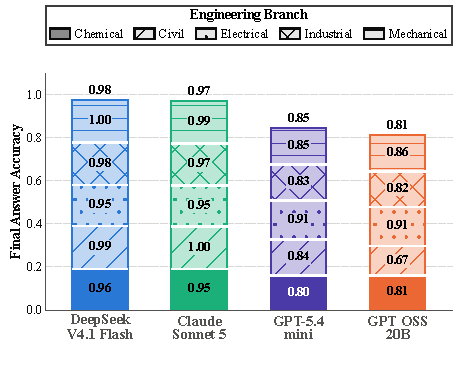
\includegraphics[width=\columnwidth]{figs/branch-bars.pdf}
    \caption{\textbf{Final Answer Accuracy by Engineering Branch for Four Representative Models.} One
    stacked bar per model, for \texttt{DeepSeek V4.1 Flash} (first on FAC), \texttt{Claude Sonnet 5}
    (first on MC), \texttt{GPT-5.4 mini}, and \texttt{gpt-oss-20b}. Each of the five branches holds 30
    of the 150 templates, so a segment is that branch's share of the model's FAC: the number inside it
    is the branch's FAC, and its height is a fifth of that. The segments add up to the model's FAC,
    printed above the bar; color marks the model and hatching the branch. The one branch pair that
    differs after Holm correction within a model is \texttt{gpt-oss-20b}'s electrical above civil
    (\autoref{tab:branch_domain}).}
    \label{fig:branch_bars}
\end{figure}
% END GENERATED fig:branch_bars

% BEGIN GENERATED fig:domain_radar (full_run_28092026/paper_results.py --write)
\begin{figure*}[t]
    \centering
    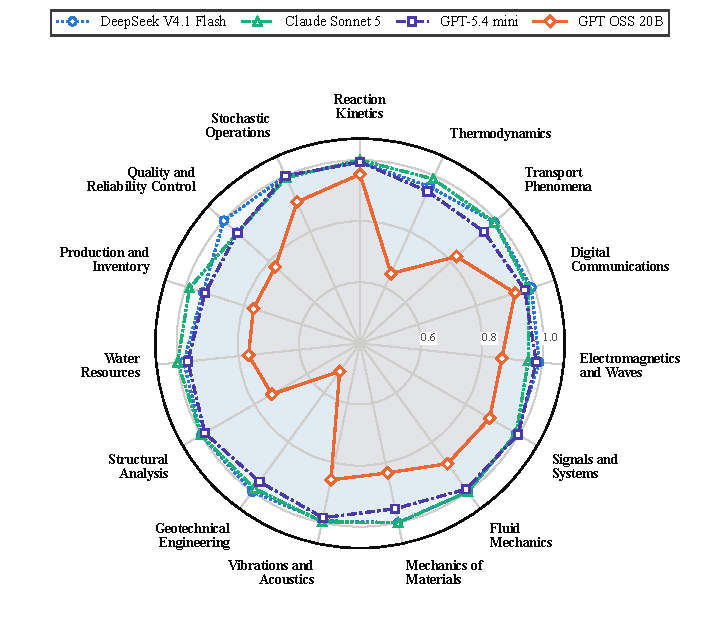
\includegraphics[width=0.74\textwidth]{figs/domain_radar/domain-radar-labeled.pdf}
    \caption{\textbf{Final Answer Accuracy by Domain for Four Representative Models.} The instance mean
    over each of the 15 domains, in the order of their branches around the rim, for the same four
    models; the radial axis starts at 0.4. The domain means carry no interval and no test
    (\autoref{tab:by_domain_kind}).}
    \label{fig:domain_radar}
\end{figure*}
% END GENERATED fig:domain_radar

% BEGIN GENERATED tab:branch_domain (full_run_28092026/paper_results.py --write)
\begin{table*}[t]
\centering
\footnotesize
\renewcommand{\arraystretch}{1.1}
\adjustbox{max width=\textwidth}{%
\begin{tabular}{l r r r r r r r r r r r }
\toprule
\rowcolor{gray!10}
\textbf{Branch or domain (templates)} & \rotatebox{90}{\texttt{DeepSeek V4.1 Flash}} & \rotatebox{90}{\texttt{Kimi K3}} & \rotatebox{90}{\texttt{Claude Sonnet 5}} & \rotatebox{90}{\texttt{GLM-5.3-Flash}} & \rotatebox{90}{\texttt{Muse Glimmer 30B}} & \rotatebox{90}{\texttt{GLM-5.3}} & \rotatebox{90}{\texttt{Qwen3-235B-2507}} & \rotatebox{90}{\texttt{Gemini 3.1 Flash-Lite}} & \rotatebox{90}{\texttt{Gemma 4 26B}} & \rotatebox{90}{\texttt{GPT-5.4 mini}} & \rotatebox{90}{\texttt{gpt-oss-20b}} \\
\midrule
\rowcolor{gray!10}\textit{Chemical} (30) & 0.956 & 0.964 & 0.949 & 0.947 & 0.963 & 0.898 & 0.827 & 0.776 & 0.734 & 0.800 & 0.809 \\
\quad Reaction kinetics (10) & 0.993 & 1.000 & 1.000 & 1.000 & 1.000 & 0.993 & 0.980 & 0.913 & 0.913 & 0.913 & 0.967 \\
\quad Thermodynamics (12) & \textbf{0.900} & 0.922 & \textbf{0.878} & \textbf{0.872} & 0.911 & \textbf{0.761} & \textbf{0.728} & \textbf{0.678} & \textbf{0.517} & \textbf{0.667} & 0.656 \\
\quad Transport phenomena (8) & 0.992 & 0.983 & 0.992 & 0.992 & 0.996 & 0.983 & 0.783 & 0.750 & 0.838 & 0.858 & 0.842 \\
\rowcolor{gray!10}\textit{Civil} (30) & 0.993 & 0.987 & 0.996 & 0.984 & 0.969 & 0.973 & 0.940 & 0.862 & 0.882 & 0.838 & 0.673$^{\ddagger}$ \\
\quad Geotechnical engineering (10) & 1.000 & 1.000 & 0.987 & 0.993 & 0.933 & 0.993 & 0.947 & 0.960 & 0.913 & 0.913 & \textbf{0.520} \\
\quad Structural analysis (10) & 1.000 & 0.993 & 1.000 & 1.000 & 0.987 & 1.000 & 0.947 & 0.913 & 0.913 & 0.827 & 0.733 \\
\quad Water resources (10) & 0.980 & 0.967 & 1.000 & 0.960 & 0.987 & 0.927 & 0.927 & 0.713 & 0.820 & 0.773 & 0.767 \\
\rowcolor{gray!10}\textit{Electrical} (30) & 0.954 & 0.949 & 0.947 & 0.981 & 0.971 & 0.951 & 0.886 & 0.900 & 0.904 & 0.911 & 0.908 \\
\quad Digital communications (10) & 0.923 & \textbf{0.897} & 0.913 & 0.967 & 0.950 & 0.923 & 0.840 & 0.877 & 0.883 & 0.923 & 0.930 \\
\quad Electromagnetics and waves (10) & 0.990 & 0.980 & 0.953 & 0.977 & 0.997 & 0.947 & 0.883 & 0.883 & 0.887 & 0.830 & 0.910 \\
\quad Signals and systems (10) & 0.950 & 0.970 & 0.973 & 1.000 & 0.967 & 0.983 & 0.933 & 0.940 & 0.943 & 0.980 & 0.883 \\
\rowcolor{gray!10}\textit{Industrial} (30) & 0.980 & 0.980 & 0.973 & 0.942 & 0.940 & 0.922 & 0.871 & 0.860 & 0.878 & 0.831 & 0.820 \\
\quad Production and inventory (10) & 0.940 & 0.967 & 0.987 & 0.887 & \textbf{0.887} & 0.887 & 0.847 & 0.853 & 0.873 & 0.780 & 0.767 \\
\quad Quality and reliability control (10) & 1.000 & 0.980 & 0.940 & 0.947 & 0.933 & 0.907 & 0.787 & 0.800 & 0.800 & 0.760 & 0.773 \\
\quad Stochastic operations (10) & 1.000 & 0.993 & 0.993 & 0.993 & 1.000 & 0.973 & 0.980 & 0.927 & 0.960 & 0.953 & 0.920 \\
\rowcolor{gray!10}\textit{Mechanical} (30) & 0.997 & 0.991 & 0.994 & 0.992 & 0.991 & 0.993 & 0.906 & 0.961 & 0.921 & 0.854 & 0.862 \\
\quad Fluid mechanics (10) & 0.997 & 0.987 & 0.987 & 0.987 & 0.987 & 0.987 & 0.913 & 0.950 & 0.893 & 0.950 & 0.880 \\
\quad Mechanics of materials (10) & 1.000 & 0.993 & 1.000 & 0.993 & 0.997 & 1.000 & 0.943 & 0.940 & 0.907 & 0.803 & 0.840 \\
\quad Vibrations and acoustics (10) & 0.993 & 0.993 & 0.997 & 0.997 & 0.990 & 0.993 & 0.860 & 0.993 & 0.963 & 0.810 & 0.867 \\
\midrule
Detectable branch difference & 0.076 & 0.072 & 0.081 & 0.089 & 0.084 & 0.126 & 0.145 & 0.182 & 0.162 & 0.182 & 0.189 \\
\bottomrule
\end{tabular}
}
\caption{\textbf{Final Answer Accuracy by Branch and by Domain.} Models in order of FAC. Shaded
rows: the mean of the branch's 30 template means; below each, its domains' instance means, which
carry no interval or test; template counts in parentheses. Bold: each model's lowest domain.
$^{\ddagger}$The one branch pair that differs within a model after Holm correction (Welch's $t$-test
over the model's ten pairs): \texttt{gpt-oss-20b}'s electrical above its civil. Last row: the
smallest branch difference 30 templates detect at 80\% power, per model.}
\label{tab:branch_domain}
\label{tab:by_branch}
\label{tab:by_domain_kind}
\end{table*}
% END GENERATED tab:branch_domain
